\documentclass[twocolumn,onesided,9pt]{article}

\usepackage{./Task32FlyerLatexStyle/Task32Flyer}
\usepackage{todonotes}
%% -----------------------------------
%% Document information
%% -----------------------------------
\def\pubdate{{24 September 2019}
\shorttitle{The OpenLidar Initiative}
\title{The OpenLidar initiative for wind lidar hardware and software collaboration}
\DOI{10.5281/zenodo.3414197}
\version{0.9}
\addbibresource{bibliography.bib}

%% ===================================
%% Document starts
%% ===================================

\begin{document}

%% -----------------------------------
%% Title
%% -----------------------------------
\maketitle
\thispagestyle{firststyle}

%% -----------------------------------
%% Introductory text
%% -----------------------------------
{\Large\noindent\nohyphens{%
Wind lidars are complex devices that take huge expertise to develop and operate. How could future lidar be designed to enable and support experimentation and collaboration?}
}
\vskip 6pt

The OpenLidar initiative was started in 2015 by members of IEA Wind Task 32. Its goal is to encourage collaboration around wind lidar hardware and software by developing a modular wind lidar architecture and providing a framework for cooperation.

\section*{Integrated solutions are not the only answer}
Wind lidar are designed and optimised for specific applications, for example to measure vertically-resolved profiles or to scan arbitrary patterns from a fixed point. They also integrate much of their function into a single unit. This focus reduces manufacturing costs and helped enabled early adoption by simplifying industry learning, but it also has some drawbacks. Such integrated systems are hard to adapt for other tasks, are usually ``black boxes'', can be over-engineered, and are hard to upgrade. As a result new applications often require entirely new devices. This need to start from scratch reduces the potential for technological innovations and makes it harder to try new applications.

\section*{The benefits of modular wind lidar}
Most wind lidar manufacturers tend to have a base design that they adapt for different uses. This reduces development costs and can speed market acceptance. For example, a scanning optics head (for following an arbitrary measurement path) could be replaced with a rotating prism to create a vertically-profiling lidar.  As a result, many lidar designs are already inherently modular. However, the module boundaries are not consistent across suppliers and so cannot be exchanged. Also, there is often little information about the data processing taking place inside the modules.

Coordinated modular lidar would allow systems to be changed and optimised depending on the lidar's use case. Modules could be developed by experts and combined by users for specific use cases. This would require well-defined interfaces between the modules for power, signals, and mounting. Ideally, vendors would also provide detailed documentation of each module.

% logo
{\centering

\includegraphics[width=0.75\linewidth]{graphics/OpenLidarLogo.png} 
}
% FH 20.09. I would suggest to put the OpenLidar logo in the header instead of having it here in the text floating around a little bit lost in between sections. This would also allow for a couple more lines or a second example in figure 2 as proposed further down.
% HF 25.09. Agree with FH. The logo should be placed in the header (or left-justified next to the two lines of the title?).

\section*{The OpenLidar concepts}
The heart of the OpenLidar initiative is the idea of modular lidar systems with clear interfaces and good documentation. Based on a survey of existing devices, the OpenLidar group developed a generic modular wind lidar architecture where the modules are connected by power and data buses (Figure \ref{fig:modules} and Table \ref{t:modules}). The function of each module can be customised for a specific application.

\begin{figure}[h]
    \centering
    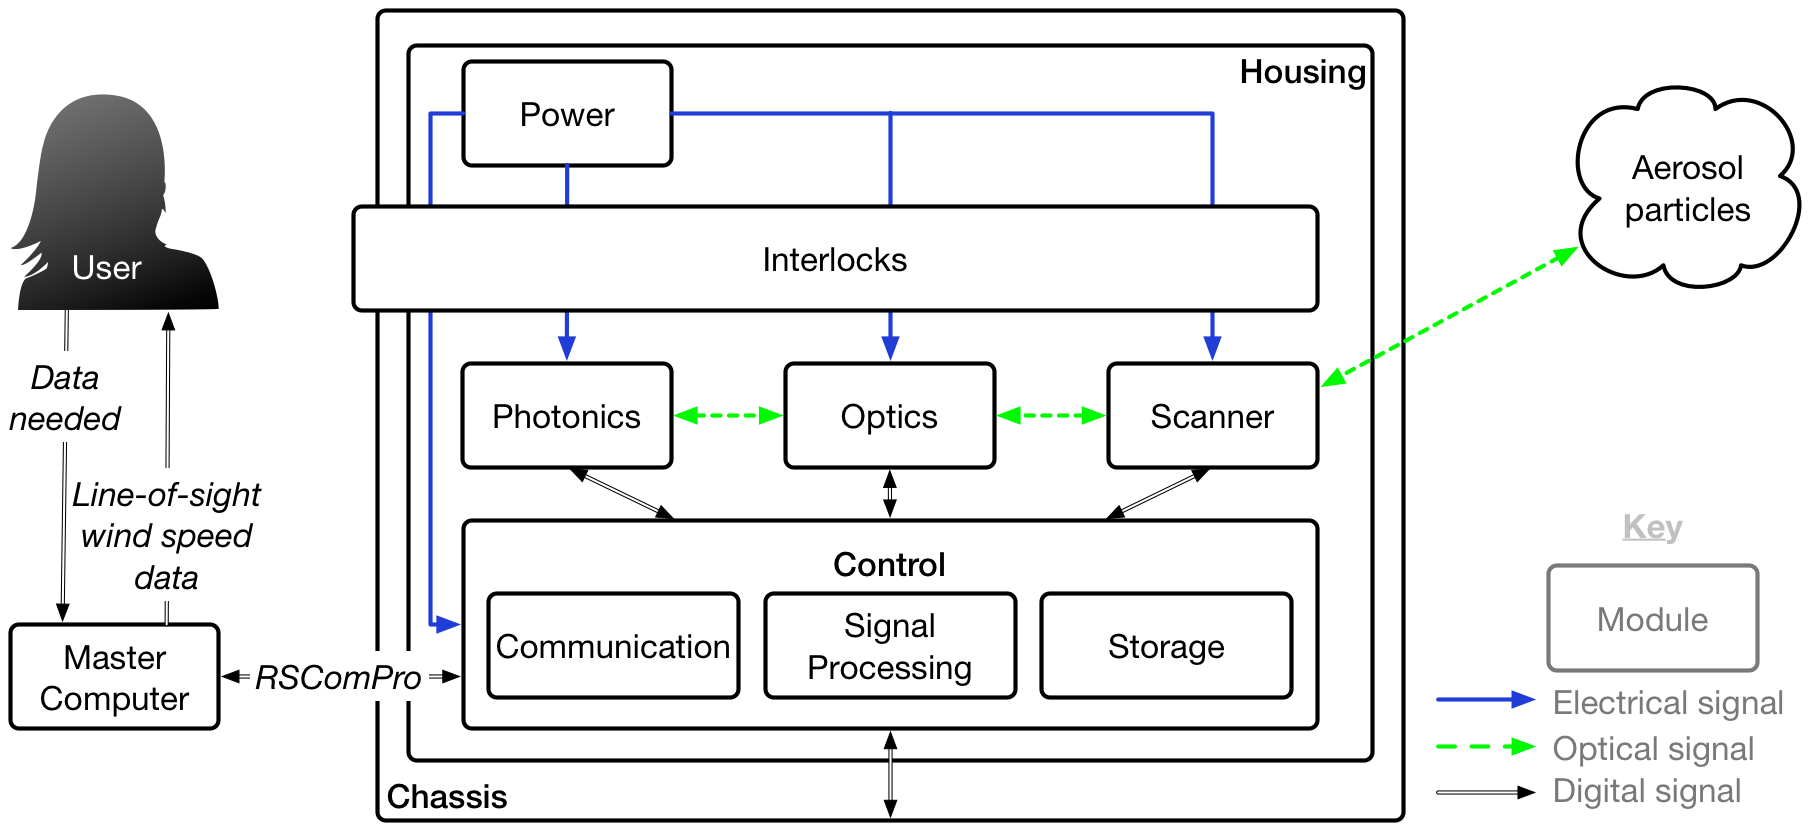
\includegraphics[width=1.1\linewidth]{graphics/OpenLidarModules.png} 
    \caption{The OpenLidar modular wind lidar concept uses digitalisation to enable innovation in wind lidar.}
\label{fig:modules}
\end{figure}

Each module requires interfaces, a module-specific controller to convert commands into action, and hardware and software to implement those commands. The modules would also be documented. These interfaces, controller, hard- and software, and documentation would allow them to be combined with other modules to create a lidar system with predictable characteristics. Importantly, such a lidar could also be modelled in detail using the design information, and those models could be validated through module unit tests.

\begin{table}[h]
	\caption{The main functions of the OpenLidar modules.}\label{t:modules}
	\begin{tabular}{@{}p{0.35\columnwidth}
			@{}p{0.65\columnwidth}@{}}
		\toprule
		Module & Function \\
		\midrule
		Power & power conversion and conditioning, current and voltage control\\
		Interlocks & safe operation of the system\\
		Photonics & Laser source, beam splitter, detector \\
		Optics & beam forming and focusing \\
		Scanner & beam steering, position sensing\\
		% HF 25.09. This is just a general comment from my point of view (maybe I should have told you that earlier): Actually I do not like "Scanner" for the name of this module. Because not every lidar has to be a scanning lidar. There are even lidars with no beam steering (see Whirlwind http://www.opticsense.eu/products-wind-lidar.php). Is a 2- or 4- beam lidar already a scanning lidar?
		% Of course we could all agree on that definition "scanner" because definitions cannot be right or wrong (only more or less useful). But somehow in my head this does not make sense. For me a scanner is only a particular subset of the lidar family, a very advanced one. Furthermore, I would subdivide lidar scanners even more accurate: into scanners with fixed or predefined scanning patterns and into scanners with "arbitrary" user-defined scanning patterns.
		% Summarising, I would break down the name of this module to a more abstract level: For me it is all about "beam deflection / steering".
		Controller & manages other modules; converts input commands to system actions\\
		Communications & transfer data to/from the device\\
		Signal processor & process raw data to e-WindLidar level 0 data \cite{Vasiljevic_2018_2478051}\\
		Storage & data memory\\
		Housing & weather protection, environmental conditioning\\
		Chassis & physical carrier(s) for modules \\
		% HF 25.09. @Andy: Please see my comment in Slack about "heating and cooling management" and "electromagnetic compatibility (EMC)". Not sure yet if those two should be own modules or if it is enough to mention them somewhere in the function column in table 1. 
		\bottomrule
	\end{tabular}
\end{table}

It is important to note that a functioning lidar does not have to be a single unit. It could also be several hardware units connected by cables for data, power, and signals. These separate units would be for e.g. the photonics, optics, and scanner (e.g. Figure \ref{fig:examples}) and there would therefore be several chassis and housing modules, each with their own interlocks.

\section*{Modular lidar in use}
The OpenLidar group set out a potential architecture for modular wind lidar in 2016. A similar architecture was used in a scanning device in 2017 \cite{Wuerth_2017_3416356}, and in 2018 a UK lidar company partnered with a University to connect a ground-based lidar to optics mounted on a drone via a glass fibre \cite{wes-2019-13}. Now, several companies supply lidar systems where the optics, photonics, and data processing units are in separate units.
% FH 20.09. Is the paper cited for the drone application actually the correct one? Isn't that Nikola's paper on the campaign planning tool?
% HF 25.09. I have just read this paper. No drones mentioned :).

\begin{figure}[h]
    \centering
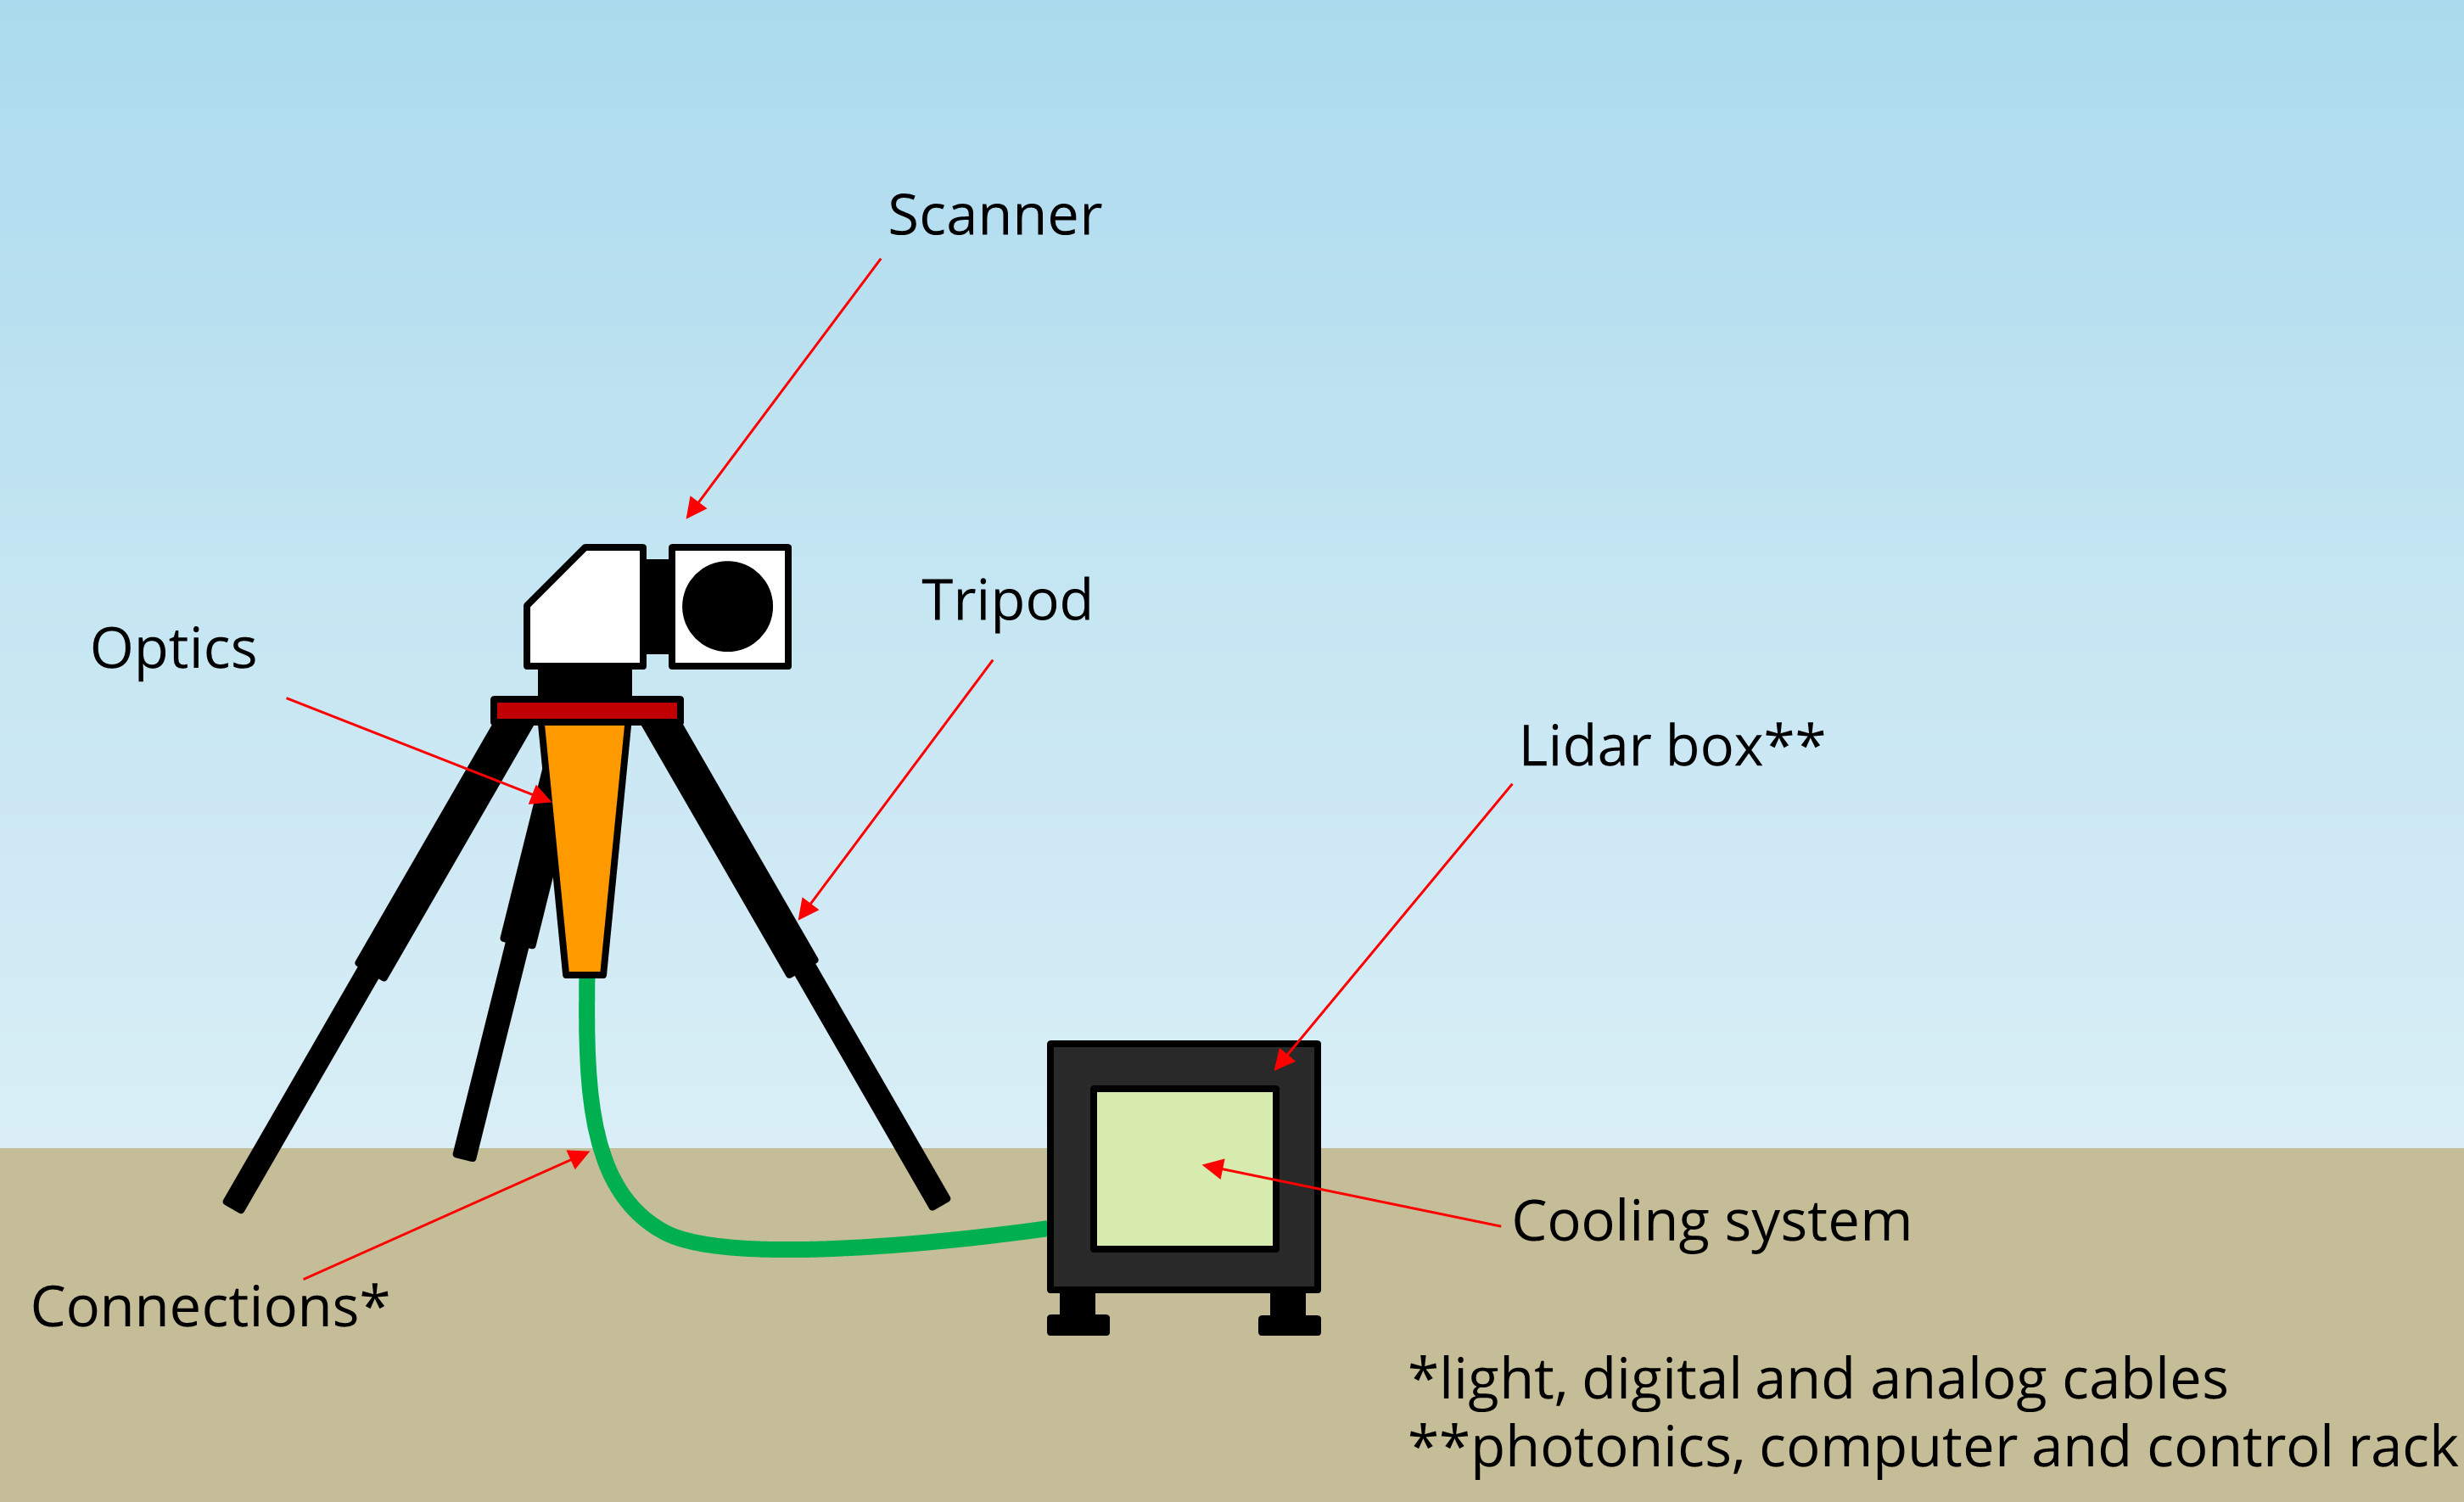
\includegraphics[width=1\linewidth]{graphics/OpenLidarExampleCropped.png} 
\caption{Openlidar modules can be combined in many ways.}
\label{fig:examples}
\end{figure}
% do we need to add a picture of a drone or a floating lidar to this?

Breaking lidar up into smaller and lighter units will lead to experiments for other applications, for example in urban meteorology, for vehicles and aviation, and elsewhere.
 
\section*{The OpenLidar development roadmap}
The IEA Wind Task 32 OpenLidar Working Group aims to support the development of modular wind lidar. This group will document the modular architecture and their interfaces, allowing vendors and other manufacturers to develop hardware and software for the modules. These hardware and software can then be used by others for new applications.

During 2020 more than 20 PhD students will start working on projects in two EU Horizon 2020 Innovative Training Networks, Lidar Knowledge Europe (ITN LIKE) and FLOAting Wind Energy NetwoRk (ITN FLOAWER). Several will apply the OpenLidar concept, adding to the body of knowledge around the development and use of modular lidar.

%documentation
Documentation will be an essential part of the OpenLidar platform. The architecture and modules are documented at \href{https://github.com/e-WindLidar/OpenLidarModuleDefinitions}{Github/e-WindLidar}. Github provides structured environment for creating the definitions and gathering feedback, and is familiar to most of the software development community. Anyone designing, building, or selling OpenLidar modules is encouraged to review these, and provide information about their modules.

\section*{Conclusions}
The OpenLidar concept aims to enable innovation and collaboration on wind lidar device hardware and software by creating a well-defined modular architecture. This is documented at Github and can be used by anyone working on wind lidar technology.

%% -----------------------------------
%% References
%% -----------------------------------
%\section*{References}
% bibliography
\label{sec:References}
\addcontentsline{toc}{section}{References}
\defbibnote{openaccess}{The following documents are all open access.}
{\small
\printbibliography[prenote=openaccess]
}

%% -----------------------------------
%% Outlined block of smaller text
%% -----------------------------------
\begin{tcolorbox}[width=1.0\columnwidth,
                  boxsep=0pt,
                  left=3pt,
                  right=3pt,
                  top=3pt,
                  arc=0pt,
                  boxrule=0.5pt,
                  toprule=0.5pt,
                  colback=white,
                  coltext=TextGrey
                  ]
{\footnotesize
This white paper was self published by IEA Wind Task 32.

%% -----------------------------------
%% IEA WIND AND TASK 32
%% -----------------------------------
\begin{tabular}{m{0.3\columnwidth}m{0.6\columnwidth}}
    % IEA Wind * DO NOT EDIT THIS TEXT *
    
\includegraphics[height=2cm]{graphics/IEAWind_logo.jpg} &
    The International Energy Agency is an autonomous organisation which works to ensure reliable, affordable and clean energy for its 30 member countries and beyond. The IEA Wind Technology Collaboration Programme supports the work of 38 independent, international groups of experts that enable governments and industries from around the world to lead programmes and projects on a wide range of energy technologies and related issues.  %
    \\
    % Task 32 * DO NOT EDIT THIS TEXT *
    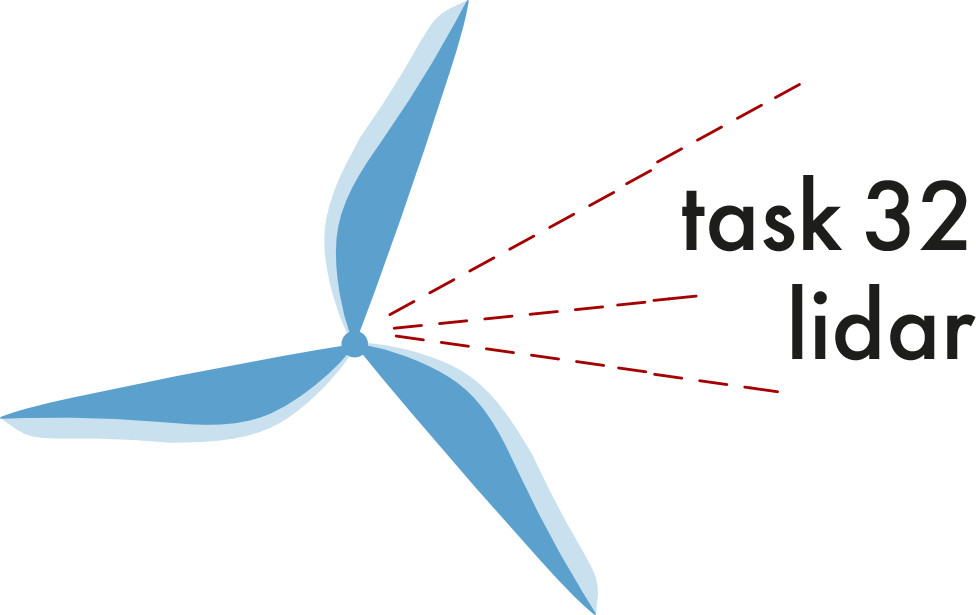
\includegraphics[height=1.5cm]{graphics/Task32_logo.jpg} &
    \href{www.ieawindtask32.org}{IEA Wind Task 32} exists to identify and mitigate the barriers to the deployment of wind lidar for wind energy applications.
\end{tabular}%

%% -----------------------------------
%% For more information
%% -----------------------------------
% N.B. do not add line breaks between the next items
\textbf{For more information:} See the  \href{https://github.com/e-WindLidar/OpenLidarModuleDefinitions}{OpenLidar module definitions on GitHub}. We welcome feedback as \href{https://github.com/e-WindLidar/OpenLidarModuleDefinitions/issues}{issues}.
%% -----------------------------------
%% Authors
%% -----------------------------------
\textbf{Authors and OpenLidar initiative team:} %
Andrew Clifton (U. Stuttgart, Germany), %
Nikola Vasiljevic (DTU Wind Energy, Denmark), %
Ines Würth (U. Stuttgart), %
Steffen Raach (U. Stuttgart \& sowento), %
Florian Haizmann (ZSW), %
Holger Fürst (U. Stuttgart).
%% -----------------------------------
%% Images
%% -----------------------------------
\textbf{Images:}
Banner, left to right: \href{https://unsplash.com/@alexkixa}{Alexandre Debiève on Unsplash}, \href{http://ifb.uni-stuttgart.de}{SWE U. Stuttgart}, \href{https://unsplash.com/@markusspiske}{Markus Spiske on Unsplash}. Figure 1 by A. Clifton. Figure 2 by N. Vasiljevic.
}

%% -----------------------------------
%% End of highlighted block
%% -----------------------------------
\end{tcolorbox}

\end{document}

% FH 20.09. Very nice and short summary of our ideas! Well done! Thanks for your efforts, Andy! (I only added two periods at the end of the captions of table 1 and figure 2.)
% HF 25.09. Ditto! Thanks Andy for pushing OpenLidar forward! 
